% Chapter 4

\chapter{Thermal front velocity in geothermal systems} % Main chapter title

\label{Chapter2} % For referencing the chapter elsewhere, use \ref{Chapter4} 

\lhead{Chapter 2. \emph{Thermal front velocity in geothermal systems}} % This is for the header on each page - perhaps a shortened title

\section{Sumary}

The injection of cold fluid into hot geothermal reservoirs can be formulated in terms of conservation laws. The cold front velocity induced during injection has been computed by Stopa and Wajnarowski in \cite{Waj05}. Their result was obtained from conservation of energy and the method of characteristics, applied to an initial boundary value problem. This computed thermal front velocity is expressed as a weighted average of the derivative of the flux function. In this paper we present a new method for computing the thermal front velocity by solving the Riemann problem. We show that the unique solution of the Riemann problem moves at the speed equal to the thermal front velocity. This result is predicted by the theory of hyperbolic conservation laws and is computed from the Rankine-Hugoniot shock condition. It is expressed as the average value of the derivative of the flux function over the interval defined by the injected water temperature and the reservoir temperature. A relative error of magnitude $10^{-3}$ was observed between the two results .%and the upper bound error of our result converges at least $133\cdot10^{4}$ times faster to zero then the one obtained in \cite{Stopa-Wajnarowski-06}. Convergence rate of about 2 was found when validating the numerical integration.

\section{Introduction}
In geothermal energy extraction, reinjecting  colder fluid into a hot reservoir is an integral part of resource management \cite{Ax-R08, Ax-Production08}. Due to the cold temperature of the injected fluid, However, cooling of the production wells can occur, as observed in Beowawe, Nevada and the Geysers Geothermal reservoir in the US  \cite{Beall}, \cite{Ben}. To mitigate this cooling effect, predicting the velocity of the cold water movement, is an essential part of the reinjection scheme. Bodvarsson \cite{Bod-R72} derived the thermal front velocity for constant fluid and rock properties, using the characteristic method. This technique produces a non physical solution when the rock and fluid properties are temperature dependent.  By using the method of characteristics, Stopa and Wajnarowski solved an initial-boundary value problem for the conservation laws \cite{Waj05}. They derived the thermal front velocity using conservation of energy. \\
\\
By formulating the injection problem as the well-posed Riemann problem, we relied on the established theory of hyperbolic conservation laws. Rather than using the method of characteristics, we used the unique solution for the Riemann problem given in \cite{Risebro07}. This solution propagates at a speed equal to the thermal front velocity.

In this work we revisit the findings of Stopa and Wajnarowski in \cite{Waj05}. In particular we compare the thermal front velocity obtained in  \cite{Waj05} with the one predicted by the theory of hyperbolic conservation laws. 
%In geothermal energy extraction, reinjecting  colder fluid into the hot reservoir is an integral part of resource management \cite{Ax-R08}, \cite{Ax-Production08}. However due to cold injected fluid, Cooling of the reservoir can occur, as observed in Beowawe, Nevada and the Geysers Geothermal reservoir in the US  \cite{Beall}, \cite{Ben}.\\
%To mitigate this cooling effect, predicting the thermal front velocity (velocity of the cold water movement), is an essential part of reinjection scheme. \\Bodvarsson \cite{Bod-R72} derived the thermal front velocity for constant fluid and rock properties, using the characteristics method. This method reduce a partial differential equation to a family of ordinary differential equation along which the solution is constant \cite{Evan00}. However for temperature dependent fluid and rock properties this method produce non physical solution. 
% \\
%Stoppa and Wajnarowski computed the thermal front velocity for temperature dependent rock and fluid properties \cite{Waj05}. They solved an initial boundary value problem by using the method of characteristics. Since this method produce non physical solution, a discontinuity was inserted into to solution such that the energy of the system was conserved. From this conservation of energy, the cold front velocity was derived.\\
% 
%In this section we present a new method for computing the thermal front velocity by solving a Riemann problem. We show that the unique solution of the Riemann problem moves at the velocity equal to the cold front velocity. Our result is computed from the Rankine-Hugoniot shock condition and is easier to evaluate using numerical integration. A difference of $10^{-8}$ was observed between our result and the one obtained in \cite{Waj05}. The upper bound error associated to our result converge rapidly to zero then the upper bound error associated to the one in \cite{Waj05} \\
%\\
%The rest of this chapter is organised as follow:
%In section 4.2 we lay down equations governing fluid flow in porous medium. Section 4.3 gives results from the theory of  hyperbolic conservation laws such as existence, and uniqueness of solution for the Riemann problem. In section 4.4 we derive the thermal front velocity for constant and temperature dependent rock and fluid properties. These derivation s are based on the theory of conservation laws from section 4.3
%


%Injection of cold fluid into a hot geothermal reservoirs can be formulated as conservation laws. The cold front velocity induced during injection has been computed by Bodvarsson \cite{Bod-R72} for constant rock and fluid properties by using the method of characteristic. This method reduce a partial differential equation to a family of ordinary differential equation along which the solution is constant \cite{Risebro07}. However for temperature dependent fluid and rock properties this method produce non physical solution. Stopa and Wajnarowski \cite{Waj05} computed the cold front velocity for temperature dependent fluid and rock properties. They solve an initial boundary value problem by using the characteristic method. Since the solution was non physical, they introduced a discontinuity at a point such that the energy of the system was conserved. From this conservation of energy, the thermal cold front velocity was derived. \\
%In this section we present a new method for computing the thermal front velocity by solving a Riemann problem. We show that the unique solution of the Riemann problem moves at the velocity equal to the cold front velocity. Our result is computed from the Rankine-Hugoniot shock condition and is easier to evaluate using numerical integration. A difference of $10^{-8}$ was observed between our result and the one obtained in \cite{Waj05}. The upper bound error associated to our result converge rapidly to zero then the upper bound error associated to the one in \cite{Waj05} \\
%
%In section 4.2 we lay down the equation governing fluid flow in porous medium. Section 4.3 gives some results from the theory of conservation laws such as existence, and uniqueness of solution for the Riemann problem. In section 4.4 we derive the thermal front velocity for constant and temperature dependent rock and fluid properties. These derivation are based on the theory of conservation laws from section 4.3
%


%%%%%%%%%%%%%%%%%%%%%%%%%%%%%%%%%%%%%%%%%%%%%%%%%%%%%%%%%%%%%%%%%%%%%%%%%%%%%%%%%%%%%%%%

\section{Governing equation}
A single phase(liquid) fluid flow in porous medium is given respectively by the conservation of mass and energy equation \cite{Woods}

\begin{equation}\label{eq:cm}
\frac{\partial (\phi \rho_{w}(u))}{\partial t} +\frac{\partial }{\partial x}(\rho_{w}(u)u_{w})=0
\end{equation}

\begin{equation}\label{eq:ce}
\phi\frac{\partial}{\partial t}\left (\phi \rho_{w}(u) c_{w}(u)u+(1-\phi)\rho_{r}(u) c_{r}(u)u\right) +\frac{\partial}{\partial x}(\rho_{w}(u) c_{w}(u) u_{w}u)=\lambda\frac{\partial^{2}u}{\partial x^{2}}
\end{equation}
\\
%-------------------------------------------------------------------------------------------------------------------------------------------------------------------------
where $u$ is the temperature, $c_{w}(u), c_{r}(u), \rho_{w}(u), \rho_{r}(u)$ are the heat capacity of water/rock and density of water/rock respectively. $\phi, u_{w}, \lambda$ are the porosity, the Darcy velocity of liquid phase and the heat conduction coefficient respectively. Darcy velocity $u_{w}$ is normally pressure dependent. Therefore equations (\ref{eq:cm}, \ref{eq:ce}) represent a system of two equations with two unknowns. \\
\\
To simplify the system of equations (\ref{eq:cm}, \ref{eq:ce}). we expend (\ref{eq:ce}) then use the conservation of mass (\ref{eq:cm}) to get one equation. See \cite{Waj05} for details. By expending (\ref{eq:ce}) we get

\begin{eqnarray}\label{eq:ce1}
c_{w}(u)u\left ( \frac{\partial \phi\rho_{w}(u)}{\partial t} +\frac{\partial }{\partial x}(\rho_{w}(u)u_{w})   \right ) + \frac{\partial }{\partial t}((1-\phi)\rho_{r}(u)c_{r}(u)u)\\ \nonumber
 + \phi\rho_{w}(u)\frac{\partial }{\partial t}(c_{w}(u)u) +  \rho_{w}(u)u_{w}\frac{\partial }{\partial x}(c_{w}(u)u) =\lambda\frac{\partial^{2}u}{\partial x^{2}}0 .
\end{eqnarray}

Using (\ref{eq:cm}), the first expression in (\ref{eq:ce1}) vanishes and we get
\begin{equation}\label{eq:ce2}
  \frac{\partial }{\partial t}((1-\phi)\rho_{r}(u)c_{r}(u)u) + \phi\rho_{w}(u)\frac{\partial }{\partial t}(c_{w}(u)u) +  \rho_{w}(u)u_{w}\frac{\partial }{\partial x}(c_{w}(u)u) =\lambda\frac{\partial^{2}u}{\partial x^{2}} .
\end{equation}
Applying the chain rule on (\ref{eq:ce2}) and assuming that Darcy velocity $u_{w}$ is constant, after rearranging the terms we end up with 
\begin{equation}\label{eq:cl}
\frac{\partial u}{\partial t} +\frac{u_{w}}{\phi}F(u)\frac{\partial u}{\partial x} =\left(\frac{\lambda}{  (1-\phi)\left( \frac{ \partial (\rho_{r}(u)  c_{r}(u) u) }{\partial u}\right) +  \phi \rho_{w}(u)\left(  \frac{\partial (c_{w}(u)u)  }{\partial u  } \right)     }\right)\frac{\partial^{2}u}{\partial x^{2}}%\frac{\partial u}{\partial t} +\frac{ \partial G }{\partial x}=0								       
\end{equation}

or 

\begin{equation}\label{eq:cl1}
\frac{\partial u}{\partial t} +\frac{ \partial G(u) }{\partial x}=\left(\frac{\lambda}{  (1-\phi)\left( \frac{ \partial (\rho_{r}(u)  c_{r}(u) u) }{\partial u}\right) +  \phi \rho_{w}(u)\left(  \frac{\partial (c_{w}(u)u)  }{\partial u  } \right)     } \right)\frac{\partial^{2}u}{\partial x^{2}}							       
\end{equation}
where 

\begin{equation}\label{eq:G0}
G(u) = \frac{u_{w}}{\phi}\int_{0}^{u}F(x)\mathrm{d}x \nonumber
\end{equation}
\begin{equation}\label{eq:F}
F(u)=\frac{  \phi \rho_{w}(u)\left(  \frac{\partial (c_{w}(u) u)  }{\partial u  }   \right)    }{  (1-\phi)\left( \frac{ \partial (\rho_{r}(u)  c_{r}(u) u) }{\partial u}\right) +  \phi \rho_{w}(u)\left(  \frac{\partial (c_{w}(u)u)  }{\partial u  } \right)     }
\end{equation}
 
 and from \cite{Waj05}
\begin{equation}
c_{w}(u)=\frac{1}{0.00023749816+8.0681767*10^{-8}u-8.0367134*10^{-10}u^{2}}\nonumber
\end{equation}
\\
\begin{equation}
c_{r}(u)=1234.257-454.546\exp(-0.00397334833482u)\nonumber
\end{equation}
\\
\begin{equation}
\rho_{w}(u)=1043.196-42.966623\exp(0.00689550122u)\nonumber
\end{equation}
\\
\begin{equation}
\rho_{r}(u)=\frac{2650}{1+(u-20)0.5*10^{-4}}.\nonumber
\end{equation}
\\

If we neglect conduction as second order effect by setting $\lambda=0$ in (\ref{eq:cl1}), we get 
\begin{equation}\label{eq:cl2}
\frac{\partial u}{\partial t} +\frac{ \partial G(u) }{\partial x}=0						       
\end{equation}
Equation (\ref{eq:cl2}) is a hyperbolic conservation laws and is the same equation derived in \cite{Waj05}. Function $G(u)$ is called the flux function of the scalar hyperbolic conservation laws. Equation (\ref{eq:cl2}) describe transport phenomenon. In this case transport of heat. Recall that $u=u(x,t)$ is the temperature and according to (\ref{eq:cl2}) the temperature is conserved. To see this, we can integrate over a given closed interval $[a,b]$ and get:
\begin{align}
\frac{\partial}{\partial t}\int_{a}^{b}u(x,t)\mathrm{d}x &=\int_{a}^{b}\frac{\partial}{\partial t}u(x,t)\mathrm{d}x\\
									      &=-\int_{a}^{b}\frac{ \partial }{\partial x}G(u(x,t))\mathrm{d}x\\
									      &=G(u(a,t))-G(u(b,t))\\
									      &=[inflow\quad at\quad a]-[inflow\quad at\quad b]
\end{align}
 Therefore the physical quantity modelled by $u$, is neither created nor destroyed: The total amount of $u$ contained inside any given interval $[a,b]$ can change only due to the flow of $u$ across boundary points $a, b$.
 \begin{figure}[H] %  figure placement: here, top, bottom, or page
    \centering
    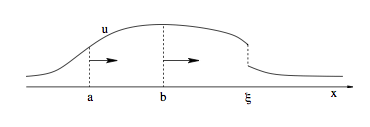
\includegraphics[width=4in]{cons.png} 
    \caption{Flow across point $a$ and $b$ with discontinuity at $\xi$}
    \label{fig:flow}
 \end{figure}
 
It is well known from the literature that equation of type (\ref{eq:cl2})  admit discontinuous solutions \cite{Risebro07}. Assume now that $u$ has a jump or discontinuity at $\xi$ see Figure \ref{fig:flow}. Then (\ref{eq:cl2}) is meaningful only in a class of discontinuous or generalised functions. Solutions must therefore be interpreted in distributional sense.
We therefore say that $u$ is a solution of (\ref{eq:cl2}) if

\begin{equation}\label{eq:weak}
\int\int( u\phi_{t}+G(u)\phi_{x})\mathrm{d}x\mathrm{d}t = 0
\end{equation}

for every infinitely continuous differentiable function $\phi$ with compact support. Equation (\ref{eq:weak}) is the weak formulation of (\ref{eq:cl2}). We only required that $u$ and $G(u)$ be locally integrable. This is a weaker requirement then continuity. To sum up, the problem of injecting colder water into a hot geothermal reservoir can be modelled by 
\begin{equation}\label{eq:cl3}
\frac{\partial u}{\partial t} +\frac{ \partial G(u) }{\partial x}=0			       
\end{equation}
with initial data
\begin{equation}\label{eq:i}
u(x,0)=u_{0}(x)						       
\end{equation}
This model assumed that the geological formation exhibit mainly micro permeability due to very small inter granular openings \cite{Bod-R72}. This mean that the reservoir is assumed homogeneous isotropic porous and permeable media, saturated with incompressible fluid. The fluid percolating through the reservoir rock. At any given point, the fluid and the reservoir have the same temperature.\\
This problem was first studied by Bodvarsson for temperature independent fluid and rock properties \cite{Bod-R72}. He found that the temperature field was transported through the porous media at a rate given by the thermal front velocity.

%Equation (\ref{eq:cl}) is a one dimension conservation laws, which can be solve with appropriate initial and/or boundary condition. In the next section, existence and unique of  (\ref{eq:cl}) is established.
%%%%%%%%%%%%%%%%%%%%%%%%%%%%%%%%%%%%%%%%%%%%%%%%%%%%%%%%%%%%%%%%%%%%%%%%%%%%%%%%%%%%%%%%






%\section{Shock wave theory for hyperbolic conservation laws}
%
%Let consider the initial value problem for Burgers equation
%\\
%\begin{equation}
%u_{t}+\left(  \frac{u^{2}}{2}\right)_{x}=0\quad in\quad \mathbb{R}\times(0,\infty), \quad u=g\quad on\quad \mathbb{R}\times(t=0)
%\end{equation}
%let the initial data $g$ be given by 
%%\begin{equation}
%\[ g(x) = \left\{ 
%  \begin{array}{l l }
%    1 & \quad \text{if $x\leq 0$ }\\
%    1-x & \quad \text{if $0\leq x\leq 1$ }\\
%    0 & \quad \text{if $x\geq 1$ }
%  \end{array} \right.\]
%%\end{equation}
%Applying the method of characteristics \cite{Evan00} the solution is given for $0\leq t\leq 1$ by 
%
%\[ u(x,t) = \left\{ 
%  \begin{array}{l l }
%    1 & \quad \text{if $x\leq t$ }\\
%    \frac{1-x}{1-t} & \quad \text{if $t\leq x\leq 1 $ }\\
%    0 & \quad \text{if $x\geq 1$ }
%  \end{array} \right.\]
%
%\begin{figure}[H] %  figure placement: here, top, bottom, or page
%   \centering
%   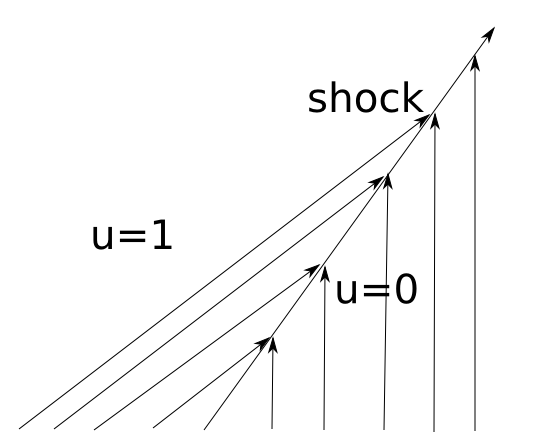
\includegraphics[width=2.5in]{sk.png} 
%   \caption{Shock wave propagation}
%   \label{fig:shock}
%\end{figure}
%
%For $t\geq 0$ the characteristics will cross and the solution is discontinuous. Now let the initial data $g$ be given by
%\[ g(x) = \left\{ 
%  \begin{array}{l l }
%    0 & \quad \text{if $x\leq 0$ }\\
%    
%    1 & \quad \text{if $x\geq 0$ }
%  \end{array} \right.\]
%
% then we can construct two solutions given by 
%\[ u_{1}(x,t) = \left\{ 
%  \begin{array}{l l }
%    0 & \quad \text{if $x\leq \frac{t}{2}$ }\\
%    
%    1 & \quad \text{if $x\geq \frac{t}{2}$ }
%  \end{array} \right.\]
%
%\[ u_{2}(x,t) = \left\{ 
%  \begin{array}{l l }
%    1 & \quad \text{if $x\leq t$ }\\
%    \frac{x}{t} & \quad \text{if $0<x< t$ }\\
%    0 & \quad \text{if $x< 0$ }
%  \end{array} \right.\]
%
%\begin{figure}[H] %  figure placement: here, top, bottom, or page
%   \centering
%   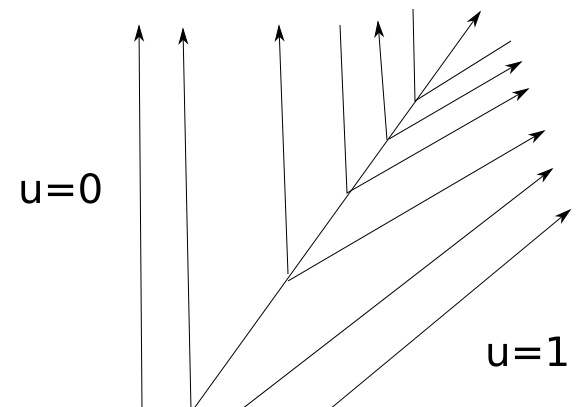
\includegraphics[width=2.5in]{u1.png} 
%   \caption{solution $u_{1}$ a non physical shock}
%   \label{fig:npshock}
%\end{figure}
%
%\begin{figure}[H] %  figure placement: here, top, bottom, or page
%   \centering
%   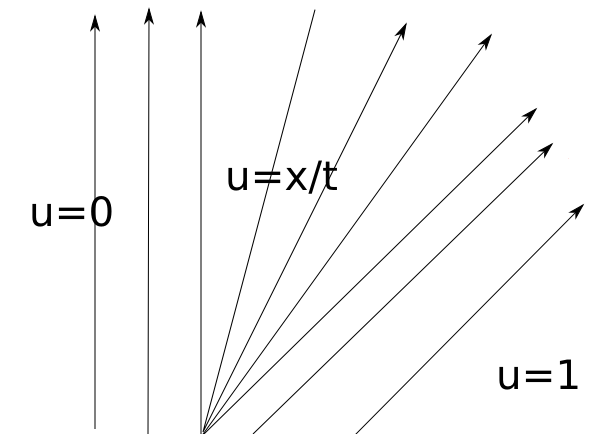
\includegraphics[width=2.5in]{u22.png} 
%   \caption{solution $u_{2}$, a rarefaction wave}
%   \label{fig:npshock}
%\end{figure}
%
%Our observation is that solutions of Burgers equation can have discontinuities with non physical shock formation. Given an initial data, the solution is not necessary unique. Under which condition can we have physical acceptable unique solution ? In the next section we set up different conditions under which the solution can be the unique physically acceptable solution.
%

%\subsection{Entropy condition and uniqueness of solution}
%The one dimension scalar conservation laws, with initial data is given by
%\\
%\begin{equation}\label{eq:conservationlaw}
%u_{t}=0\quad u(x,0)=u_{0}.
%\end{equation}
%\\
%Integrating (\ref{eq:conservationlaw}) between two points $x_{1}$ and $x_{2}$  we get
%\\
%\begin{align*}
%\frac{d}{dt}\int_{x_{1}}^{x_{2}} u(x,t)dx &=F(u(x_{1},t))-F(u(x_{2},t))\\
%                                                                   &=[inflow\quad at\quad x_{1}]-[outflow\quad at\quad x_{2}]. \nonumber
%\end{align*}
%\\
%Equation (\ref{eq:conservationlaw}) expresses the conservation of the quantity measured by $u$, since the rate of change of the amount of $u$ between $x_{1}$ and $x_{2}$ is given  by the difference in $F(u)$ evaluated at those points.This suggest that $F(u)$ should be interpreted as the flux of $u$ at the boundary points. In the theory of partial differential equation, it is common practice to seek weak solution then try to prove that the weak solution is differentiable. The differentiability of weak solution are expressed in term of weak derivatives. By following those steps, we start by laying down the weak formulation of the conservation law. This procedure is dictated by the physical phenomenon that (\ref{eq:conservationlaw}) model. As mention before conservations laws model shock wave propagation, and since shock waves induce discontinuity in the physical characteristics of the medium though which they propagate, one should expect the temperature profile of (\ref{eq:conservationlaw}) to be discontinuous.
%
%When $F(u)^{\prime}$ in (\ref{eq:conservationlaw}) dependent on temperature $u$, (\ref{eq:conservationlaw}) is non-linear, and continuous solutions do not exist. One is therefore forced to extend the solution set to generalized function or distribution (weak solution).\\
%A distribution $g$ is a continuous linear functional on $C_{0}^{\infty}$ (the space of infinitely differentiable function) such that for any family $\varphi_{n}$ $\in$ $C_{0}^{\infty}$ with supp$\varphi_{n}$ $\subseteq$ $K$, where $K$ is compact and such that all derivative satisfy $\varphi^{(m)}_{n}$ $\rightarrow$ $\varphi^{(m)}$ uniformly for some $\varphi$ $\in$ $C_{0}^{\infty}$, we have $g(\varphi_{n})$:= $\left <g,\varphi_{n}\right >$ $\rightarrow $ $\left <g,\varphi \right >$ . A function $\varphi$ $\in$ $C_{0}^{\infty}$ is generally called a test function.\\
%Our goal is to now give a formal definition of what it mean for $u$ to be a distribution or weak solution of (\ref{eq:conservationlaw}). Incorporating initial condition into the definition of weak solution, we define the partial derivative of a weak solution $u$ with respect to $t$ as:
%\begin{equation}\label{eq:weaks}
%\left<u_{t},\varphi\right>:=\int_{-\infty}^{\infty} u(x,0)\varphi(x,0)\mathrm{d}x -\left<u,\varphi_{t}\right>.
%\end{equation}
%And since the weak solution $u$ is defined for almost all $x$ and $t$, we get:
%\begin{eqnarray}
%  0& = & \left<0,\varphi \right> \nonumber \\
%   & = & \left<u_{t}+F(u)_{x},\varphi \right> \nonumber\\
%   & = & -\int_{-\infty}^{\infty}u(x,0)\phi(x,0)\mathrm{d}x-\left<u,\varphi_{t}\right>-\left<f(u),\phi_{t}\right> \nonumber \\
%   & = & \int_{-\infty}^{\infty}\int_{0}^{\infty}\left(u\varphi_{t}+F(u)\varphi_{x}\right) \mathrm{d}t \mathrm{d}x-\int_{-\infty}^{\infty}u(x,0)\varphi(x,0)\mathrm{d}x,
%\end{eqnarray}
%
%for all test function $\varphi$.\\
%The next definition gives a formal formulation of weak solution of the conservation laws.
%\begin{definition}
%Let $f:\mathbb{R} \longrightarrow \mathbb{R}$ be a smooth function. A measurable function $u=u(x,t)$, defined on an open set $\Omega \subseteq \mathbb{R}\times \mathbb{R}$ and with values in $\mathbb{R}$ is a weak solution or distributional solution of the conservation laws , if for every test function $\varphi :\Omega \longrightarrow \mathbb{R}$ with compact support, (\ref{eq:weaks}) is satisfied.
%\end{definition}
%Observe that no continuity assumption is made on the the weak solution $u$. The only requirement is that $u$ and $f$ be locally integrable: $u$, $f(u)$ $\in L_{loc}^{1}$.\\
% Next we investigate the type of weak solutions that satisfies (\ref{eq:weaks})). We keep in mind that our ultimate goal is to show that there exist a unique solution to the conservation law, and that this unique solution is stable with respect to the initial data. This last condition is very important for any physical application.\\
% 
 
 %%%%%%%%%%%%%%%%%%%%%%%%%%%%%%%%%%%%%%%%%%%%
%To prove uniqueness of solution a condition derived from physical experience called entropy condition must be imposed on equation (\ref{eq:conservationlaw})). This is done since there exist many solutions and we need to filter those solutions in order to capture the physical admissible one. Imposing an entropy condition on the conservation law lead to the so called Rankine-Hugoniot jump condition, which is an extra condition that a shock wave must posses. It gives the propagation speed of the shock wave across a discontinuity. We express all this formally as followed: we know that the physical problem that (\ref{eq:conservationlaw})) model has viscosity, and the conservation laws that is derive is the limit of the real physical phenomenon. The entropy condition is then called the viscous regularisation or \emph{traveling wave entropy condition} \cite{Risebro07}. Since the conservation laws is the limit of
%
%\begin{equation}\label{eq:viscousity}
%u_{t}^{\epsilon} + F(u^{\epsilon})_{x} = \epsilon u_{xx}^{\epsilon},
%\end{equation}
%as $\epsilon$ $\rightarrow$ $0$, where $\epsilon$ is nonnegative. Equation(\ref{eq:viscousity}) is well-posed classically, meaning that its exist a unique smooth solution and that the solution is stable with respect to the initial data. Suppose that the solution $u$ move with a speed $s$ across the discontinuity with a constant state:
%
%\begin{equation}
%u(x,t) = \left\{
%\begin{array}{rl}
%u_{l} & \text{if } x < st\\
%u_{r} & \text{if } x \geq st.
%\end{array} \right.
%\end{equation}
%
%Let $u^{\epsilon}=U((x-st)/ \epsilon)=U( \xi)$ be the solution of (\ref{eq:viscousity}). By definition, $u$ satisfy \emph{the traveling wave entropy condition} if $u(x,t)=u^{\epsilon}(x,t)=U(\xi)$ as $\epsilon$ goes to 0 pointwise.
%Now inserting $u^{\epsilon}$ into (\ref{eq:viscousity}) gives:
%\begin{equation}
%-s\dot{U}+\frac{dF(U)}{d\xi}=\ddot{U}.
%\end{equation}
%And integrating gives:
%
%\begin{equation}\label{eq:rankine}
%\dot{U}=-sU+F(U)+A.
%\end{equation}
%Since $u(x,t)$ satisfy the \emph{traveling wave entropy condition} we have:
%
%\begin{equation}
%U(\xi) = \left\{
%\begin{array}{rl}
%u_{l} & \text{if } x < st\\
%u_{r} & \text{if } x \geq st.
%\end{array} \right.
%\end{equation}
%as $\epsilon$ goes to 0, which yield $\dot{U(\xi)}=0$ as $\xi$ goes to infinity. Inserting this in (\ref{eq:rankine}) yield
%\begin{equation}\label{eq:rhugoniot}
%s(u_{l}-u_{r})=F(u_{l})-F(u_{r})
%\end{equation}
%which is the Rankine-Hugoniot jump condition. We formally express this in the following lemma.
%
%\begin{lemma}
%If the function $u=u(x,t)$ is the solution of the conservation laws with initial data,
%\begin{equation}
%u(x,0) = \left\{
%\begin{array}{rl}
%u_{l} & \text{if } x <0\\
%u_{r} & \text{if } x \geq0
%\end{array} \right.
%\end{equation}
%Then (\ref{eq:rhugoniot}) hold.
%\end{lemma}
%
%\begin{proof}
%See \cite{Risebro07}, page 9-11.
%Let $\varphi$ be a test function, and let $\Omega$ be a ball containing the support of $\varphi$. We consider the two domains:\\
%$\Omega^{+}=\Omega\cup \{x>st\}$, \quad $\Omega^{-}=\Omega\cup \{x<st\}$, where st is the line through the origin of the $(x,t)$ plane, separating $\Omega$ into $\Omega^{+}$ and $\Omega^{-}$. We introduce the vector field $\textbf{V}=(u\varphi, F(u)\varphi)$, so that,
%\begin{equation}
%\iint_{\Omega^{+}\cup\Omega^{-}}\nabla.\textbf{V}\mathrm{d}x\mathrm{d}t=0.
%\end{equation}
%Let $\textbf{n}^{+}$ and $\textbf{n}^{-}$ denote the outer unit normal to $\Omega^{+}$ and $\Omega^{-}$ respectively. Let $dS$ denote the differential of the arc length along the line $x=st$. We then have:\\
%$\textbf{n}^{+}dS=(s,-1)dt$,\quad\quad $\textbf{n}^{-}dS=(-s,1)dt$.\\ Applying Guauss theorem respectively to $\Omega^{+}$ amd $\Omega^{-}$, we get:
%
%\begin{equation}
%\begin{aligned}
%\iint_{\Omega^{+}\cup\Omega^{-}}\nabla.\textbf{V}\mathrm{d}x\mathrm{d}t&=\int_{\partial\Omega^{+}}\textbf{n}^{+}.\textbf{V}\mathrm{d}S+\int_{\partial\Omega^{-}}\textbf{n}^{+}.\textbf{V}\mathrm{d}S\\
%                                                                       &=\int\left[su_{r}-F(u_{r})\right]\varphi(st,t)\mathrm{d}t+\int\left[-su_{l}+f(u_{l})\right]\varphi(st,t)\mathrm{d}t\\
%                                                                       &=\int\left[s(u_{r}-u_{l})-F(u_{r})-F(u_{l})\right]\varphi\mathrm{d}t=0                                                                      
%\end{aligned}
%\end{equation}
%which implies (\ref{eq:rhugoniot}).
%\end{proof}
%An other entropy condition (condition derived from physical laws) called the \emph{Kruzkov entropy condition} is important in the sense that it incorporate the definition of weak solution, and is an important tool in proving the uniqueness of the conservation laws. It is given for the time interval $[0,T]$ in the integral form as followed:
%
%\begin{equation}
%\int_{0}^{T}\int_{-\infty}^{\infty}\left( \mid u-k \mid \varphi_{t}+q(u,k)\varphi_{x} \right) \mathrm{d}x \mathrm{d}t + \int \mid u(x,0)-k \mid \varphi(x,0) \mathrm{d}x  \geq 0 
%\end{equation}
%\\
%where $q(u,k)=sign(u,k)(F(u)-F(k))$, $k$ is a non negative constant and $\varphi$ is any non negative test function.
%We note that the \emph{traveling wave entropy condition} and the \emph{Kruzkov entropy condition} are equivalent for sufficiently smooth weak solution. We introduce a lemma which is needed to prove uniqueness.
%
%\begin{lemma} see,\cite{Risebro07}.
%let $h$ $\in$ $L^{\infty}(\mathbb{R\times R})$ with compact support. Assume that for almost all $x_{0} \in \mathbb{R}$ the function $h(x,y)$ is continuous at $(x_{0},x_{0})$. The following hold:
%\begin{equation}
%lim_{\epsilon \rightarrow 0}\int\int h(x,y)w_{\epsilon}(x-y)\mathrm{d}y\mathrm{d}x =\int h(x,y)\mathrm{d}x.
%\end{equation}
%\end{lemma}
%
%
%Now we are ready to prove the following theorem giving the uniqueness of solution.
%\begin{theorem} see \cite{Risebro07}.
%Assume that $F$ is Lipschitz continuous, and let $u$ and $v$ be two weak solutions of the initial value problems
%\begin{equation}
%u_{t}+F(u)_{x}=0 \quad u(x,0)=u_{0}
%\end{equation}
%\begin{equation}
%v_{t}+F(v)_{x}=0 \quad v(x,0)=v_{0}
%\end{equation}
%respectively satisfying the \emph{Kruzkov entropy condition} . Assume that $u_{0}-v_{0}$ is integrable and both $u$ and $v$ have finite total variation in $x$ for each $t$. Then
%\begin{equation}
%\mid\mid u(x,t)-v(x,t) \mid\mid_{1}\quad \leq\quad\mid\mid u_{0}-v_{0} \mid\mid_{1}
%\end{equation}
%In particular, if  $u_{0}=v_{0}$ then $u=v$.
%\end{theorem}
%
%\begin{proof}
%To prove \textbf{Theorem 2} we assume that there exist a constant $C$ such that the following is satisfy:
%
%\begin{equation}
%sup\frac{\mid F(u)-F(v)\mid}{\mid u-v\mid} \leq C
%\end{equation}
% For $u \neq v$. We assume also that $u$ and $v$ are of bounded variation in $x$ for each fixed $t$ that is 
% 
% \begin{equation}
% T.V.(u(.,t)),T.V.(v(.,t))<\infty
% \end{equation}
% 
% Where $T.V.(u)=sup \sum_{i}( u(x_{i})-u(x_{i-1}))$ and the supremum is taken over any finite partition. Consequently if $u$ is of bounded variation then $u$ is continuous almost every where in distribution. Now since $u$ and $v$ are weak solutions of the conservation laws, they satisfy the \emph{Kruzkov entropy condition (KEC)} . Assume also that the test function $\varphi$ is compactly supported in $t>0$, then KEC becomes:
%
% \begin{equation}
%\int_{0}^{t}\int_{-\infty}^{\infty}\left( \mid u-k \mid \varphi_{t}+q(u,k)\varphi_{x} \right) \mathrm{d}x \mathrm{d}t \geq 0 
%\end{equation}
%Now we use the method of doubling of variable. We double the variable of the test function $\varphi(x,t)$ to $\varphi(x,t,y,s)$ compact supported in $t>0$ and $s>0$. This smart choice of the test function $\varphi$ is important. Let $\psi(x,t)$ be an other test function with compact support in $t>\epsilon_{0}$ such that:
%\begin{equation}
%\varphi(x,t,y,s)=\psi\left(\frac{x+y}{2},\frac{t+s}{2}\right)w_{\epsilon_{0}}(t-s)w_{\epsilon}(x-y)
%\end{equation}
%And we get:
%
%\begin{equation}
%\varphi_{t}+\varphi_{s} = \psi_{t}\left(\frac{x+y}{2},\frac{t+s}{2}\right)w_{\epsilon_{0}}(t-s)w_{\epsilon}(x-y)
%\end{equation}
%
%
%\begin{equation}
%\varphi_{x}+\varphi_{y} = \psi_{x}\left(\frac{x+y}{2},\frac{t+s}{2}\right)w_{\epsilon_{0}}(t-s)w_{\epsilon}(x-y)
%\end{equation}
%
%Since both $u$ and $v$ satisfies the \emph{Kruzkov entropy condition}, we set $k=u(x,t)$ in the expression for $u$ and $k=v(y,s)$ in the expression for $v$ in the KEC formulation, and this gives us:
%
%\begin{equation}
%\iiiint(\mid u(x,t)-v(y,s) \mid(\varphi_{t}+\varphi_{s})+q(u,v)(\varphi_{x}+\varphi_{y}))\mathrm{d}x\mathrm{d}t\mathrm{d}y\mathrm{d}s \geq 0
%\end{equation}
%
%Assume now that $\psi$ is supported in $t>\epsilon$, and we want to apply \textbf{lemma1} respectively to $h(x,t)=\mid u(x,t)-v(y,s)\mid w_{\epsilon_{0}}(\phi_{t}+\phi_{s})$ and $h(x,y)=q(x,y)w_{\epsilon_{0}}(\phi_{x}+\phi_{y})$, this is justify since we fix $t$ and $s$, and therefore $u$ and $v$ are only functions of $x$ and $y$. Now by letting $\epsilon_{0}$ and $\epsilon$ goes to 0 and applying \textbf{lemma 2}, we get
%
%\begin{equation}
%\iint(\mid u(x,t)-v(x,t)\mid \psi_{t} +q(u,v)\psi_{x}) \geq 0.
%\end{equation}
%
%If the time variable in $u(x,t)$ is in the time interval [0,T], the \emph{Kruzkov entropy condition} becomes:
%\begin{equation}\label{eq:kec0}
%\int_{0}^{T} \int \mid u-k \mid \varphi_{t} +q(u,k)\varphi_{x} \mathrm{d}x \mathrm{d}t-\int\mid u(x,T)-k \mid \varphi(x,T)\mathrm{d}x+\int \mid u_{0}(x)-k \mid \varphi(x,0)\mathrm{d}x \geq 0.
%\end{equation}
%For any test function $\varphi$ $\in$ $C_{0}^{\infty}\left(\mathbb{R} \times [0,T]\right)$ and all nonnegative real $k$.
%
%If the support of $\varphi$ include $0$ and $T$, the \emph{Kruzkov entropy condition} becomes:
%
%\begin{equation}\label{eq:kec1}
%\begin{aligned}
%&  \iiiint(\mid u(x,t)-v(y,s) \mid)(\varphi_{t}+\varphi_{s})+q(u,v)(\varphi_{x}+\varphi_{y}))\mathrm{d}x\mathrm{d}t\mathrm{d}y\mathrm{d}s\\
%&-\iiint \mid u(x,T)-v(y,s)\mid \varphi(x,T,y,s)\mathrm{d}x\mathrm{d}y\mathrm{d}s\\
%&-\iiint \mid u(x,T)-v(y,s)\mid \varphi(x,T,y,s)\mathrm{d}x\mathrm{d}y\mathrm{d}t\\
%&+\iiint \mid u_{0}(x)-v(y,s)\mid \varphi(x,0,y,s)\mathrm{d}x\mathrm{d}y\mathrm{d}s\\
%&+\iiint \mid u(x,t)-v_{0}(y)\mid \varphi(x,t,y,0)\mathrm{d}x\mathrm{d}y\mathrm{d}t \geq 0.
%\end{aligned}
%\end{equation}
%When $s \rightarrow t$ and $y \rightarrow x$ we get:
%
%\begin{equation}
%\begin{aligned}
%& \iint (\mid u(x,t)-v(x,t)\mid \psi_{t}+q(u,v)\psi_{t})\mathrm{d}t\mathrm{d}x\\
%&-\int \mid u(x,T)-v(x,T)\mid \psi(x,T)\mathrm{d}x\\
%&+\int \mid u_{0}(x)-v_{0}(x)\mid \psi(x,0)\mathrm{d}x \geq 0.
%\end{aligned}
%\end{equation}
%Next we express the test function $\psi$ as the convolution of the characteristics function $\chi$ of the interval $[-M+Ct+\epsilon,M-Ct-\epsilon]$ and the function $w_{\epsilon}$. The constant $M$ is chosen such that $\psi$ is an admissible test function, in other word: $ \psi(x,t)=\left(\chi_{[-M+Ct+\epsilon,M-Ct-\epsilon]}*w_{\epsilon}\right)(x)$.  For $t\in [0,T]$, we get:
%\begin{equation}
%\begin{aligned}
%\varphi_{t}&=\frac{d}{dt}\int_{-M+Ct+\epsilon}^{M-Ct-\epsilon} w_{\epsilon}(x-y)\mathrm{d}y\\
%        &=-C\left(w_{\epsilon}(x-M+Ct+\epsilon)-w_{\epsilon}(x+M-Ct-\epsilon)\right)        
%\end{aligned}
%\end{equation}
%And in the same way we get :
%\begin{equation}
%\psi_{x}= -\left(w_{\epsilon}(x-M+Ct+\epsilon)-w_{\epsilon}(x+M-Ct-\epsilon)\right)
%\end{equation}
%So that:
%\begin{equation}
%\psi_{t}+\frac{q(u,v)}{\mid u-v \mid}\psi_{x} \leq \psi_{t}+C\psi_{x} =0
%\end{equation}
%which implies:
%\begin{equation}
%\mid u-v \mid \psi_{t}+q(u,v)\psi_{x} \leq 0
%\end{equation}
%Leting $\epsilon \rightarrow 0$, we have, 
%\begin{equation}
%\int_{-M+Ct}^{M-Ct} \mid  u(x,t)-v(x,t)\mid \mathrm{d}x \leq \int_{-M}^{M} \mid u_{0}(x)-v_{0}(x) \mid \mathrm{d}x
%\end{equation}
%which implies:
%
%\begin{equation}
%\mid\mid u(x,t)-v(x,t)\mid\mid_{1} \leq \mid\mid u_{0}-v_{0}\mid\mid_{1}
%\end{equation}
%\end{proof}
%And the above expression express stability in $L^{1}$, therefore uniqueness of solution. 
%The conservation law (\ref{eq:conservationlaw}) therefore is well posed in the sense of distribution and its solution is given in the next section.
%
%
%\subsection{Solution of the conservation law}
%The solution of the conservation laws given for the Riemann problem,
%
%\begin{equation}\label{eq:rieman}
%u_{t}+F(u)_{x}=0,\quad 
%u(x,0) = \left\{
%\begin{array}{rl}
%u_{l} & \text{if } x <0\\
%u_{r} & \text{if } x \geq0
%\end{array} \right.
%\end{equation}
% depend on the values of $u_{l}$ and $u_{r}$. We now state a theorem giving the solution of of the Riemann problem for the conservation laws, but we need to introduce a definition first.
%\begin{definition}
% The lower convex envelope of $F$ denoted by $F_{\cup}$ in the interval $[u_{l},u_{r}]$ is the largest convex function that is smallest than or equal to $f$in the interval $[u_{l},u_{r}]$. And the upper concave envelope denoted by $F_{\cap}$ is defined to be the smallest concave function that is bigger than or equal to $F$ in the interval $[u_{l},u_{r}]$. 
%\end{definition}
%
% 
%\begin{theorem}
%The initial value problem (\ref{eq:rieman}) with flux function $F(u)$ such that $F_{\cup},_\cap \neq f$ on finitely many intervals alternating with interval where they coincide, has a weak solution given by:
%\begin{equation}
%u(x,t) = \left\{
%\begin{array}{rl}
%u_{l} & \text{if } x \leq F^{\prime}_{\cup}(u_{l})t,\\
%(F^{\prime}_{\cup})^{-1}(\frac{x}{t}) & \text{if }F^{\prime}_{\cup}(u_{l})t\leq x \leq F^{\prime}_{\cup}(u_{r})t\\
%u_{r} & \text{if } x \geq F^{\prime}_{\cup}(u_{r})t
%\end{array} \right.
%\end{equation}
%If $u_{l}<u_{r}$, and:
%\begin{equation}
%u(x,t) = \left\{
%\begin{array}{rl}
%u_{l} & \text{if } x \leq f^{\prime}_{\cap}(u_{l})t,\\
%(F^{\prime}_{\cap})^{-1}(\frac{x}{t}) & \text{if }F^{\prime}_{\cap}(u_{l})t\leq x \leq F^{\prime}_{\cap}(u_{r})t\\
%u_{r} & \text{if } x \geq F^{\prime}_{\cap}(u_{r})t
%\end{array} \right.
%\end{equation}
%if $u_{l}>u_{r}$
%\end{theorem}
%
%
%We only give the sketch of the proof. For details of the proof see \cite{Risebro07}.
%\begin{proof}
%We must show that the \emph{Kruzkov entropy condition} is satisfied. This must be so since the function $u(x,t)$  is the unique weak solution of of the conservation law. Recall that any unique weak solution must satisfy the \emph{Kruzkov entropy condition}. The solution for the Riemann problem of the conservation law is invariant under the transformation $x\rightarrow kx$ and $t\rightarrow kt$. We then look for solution of the form:$u=u(x,t)=h(\frac{x}{t})=h(z)$. When we introduce this equality into the conservation law and simplify, we get: 
%\begin{equation}
%z=F^{\prime}(h).
%\end{equation}
%If the flux function $F$ is strictly monotone, we can invert the relation $Z$ and obtain:
%
%\begin{equation}
%h=(F^{\prime})^{-1}(z).
%\end{equation}
%However this is not generally the case. To solve this problem, we have to replace $F^{\prime}$ by a monotone function in the interval $[u_{l},u_{r}]$. And those monotone functions are either given by the lower convex envelope $F^{\prime}_{\cup}$ or the upper concave envelope $F^{\prime}_{\cap}$.We set $s_{i}=F^{\prime}_{\cup}(u_{i})$ and define $s_{0}=-\infty$ and $s_{n+1}=\infty $. We assume that $s_{0}<s_{1}<...<s_{n+1}$.Define the solution $u_{i}(x,t)$ on each interval $s_{i-1} \leq \frac{x}{t} \leq s_{i}$ by:
%\begin{equation}
%u_{i}(x,t)=(F^{\prime}_{\cup})^{-1}\left (\frac{x}{t}\right)
%\end{equation}
%for $i=2,...,n$,
%where $u_{1}(x,t)=u_{l}$ for $x\leq s_{1}t$ and $u_{n+1}(x,t)=u_{r}$, for $x\geq s_{n}t$. By introducing the set 
%\begin{equation}
%\Omega_{i}=\{(x,t), 0\leq t \leq T\}
%\end{equation}
%for $s_{i-1}<x<s_{i}$, the solution $u(x,t)$ is then given by:
%\begin{equation}
%u(x,t)=\sum_{i}^{n+1}{\chi_{\Omega_{i}}(x,t)u_{i}(x,t)},
%\end{equation}
%where $\chi_{\Omega_{i}}$ is the characteristics function of the set $\Omega_{i}$. Next we set $\eta_{i}=\mid u_{i}-k\mid$ and $q_{i}=sign(u_{i}-k)(f(u_{i}-f(k))$. For $k$ not between $u_{l}$ and $u_{r}$ the Rankine-Hugoniot jump condition hold and we have:
%\begin{equation}
%s_{i}(\eta_{i}(u_{l})-\eta_{i}(u_{r}))=q_{i}(u_{l})-q_{i}(u_{r}).
%\end{equation}
%For $k$ between $u_{l}$ and $u_{r}$, The \emph{Kruzkov entropy condition hold and we have}:
%
%\begin{equation}
%s_{i}(\eta_{i}(u_{l})-\eta_{i}(u_{r}))\geq q_{i}(u_{l})-q_{i}(u_{r}).
%\end{equation}
%Applying Gauss theorem on each $\Omega_{i}$, the \emph{Kruzkov entropy solution }  is satisfy and $u$ is en entropy solution, therefore a weak solution, of the Riemann problem.
%\end{proof}
%
%



%%%%%%%%%%%%%%%%%%%%%%%%%%%%%%%%%%%%%%%%%%%%%%%%%%%%%%%%%%%%%%%%%%%%%%%%%%%%%%%%%%%

\section{Thermal front velocity}
\subsection{Formulation of the problem and early work}
We consider a geothermal reservoir with temperature $u_{r}$  and a flash water from geothermal power plant of temperature $u_{l}$. Assume that $u_{l}<u_{r}$. The flash water is injected into the reservoir. We are interested in finding the rate at which the colder injected water propagates through the reservoir. Ultimately we can calculate the distance traveled by the cold injected water with time. The thermal front velocity is defined as the rate at which the cold injected fluid moves through the reservoir rock.

Bodvarsson formulated this problem for constant rock and fluid properties \cite{Bod-R72} by

\begin{equation}
\frac{\partial u}{\partial t} +w\frac{ \partial u }{\partial x}=0	\nonumber		       
\end{equation}
with solution
\begin{equation}
u = f(x-wt)  \nonumber
\end{equation}
which means that the temperature filed is translated with velocity $w$ (thermal front velocity), given an initial data 
\begin{equation}
u(x,0) = f(x) \nonumber
\end{equation}
In the injection problem the initial data $f(x)$ is given as a step function see figure \ref{fig:tf1}. Due to the simplicity of the problem, he was able to apply  this method to cylindrical and spherical symmetric flow.
\\
Since solution of (\ref{eq:cl2}) admit discontinuities, practically the thermal front velocity is the velocity of the discontinuity solution.
\begin{figure}[H] %  figure placement: here, top, bottom, or page
   \centering
   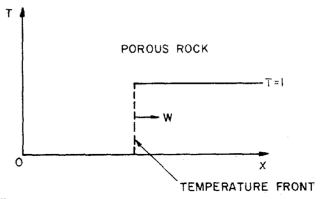
\includegraphics[width=4in]{tf1.png} 
   \caption{Thermal front moving with velocity $w$ through a porous rock}
   \label{fig:tf1}
\end{figure}
\\
Two cases can be considered. In the first case the rock and fluid properties are assumed constant. In this case equation (\ref{eq:cl3}) becomes:
\begin{equation}
\frac{\partial u}{\partial t}+\left( \frac{u_{w}}{\phi} \frac{\phi\rho_{w}c_{w}}{(1-\phi)\rho_{r}c_{r}+\phi\rho_{w}c_{w}} \right)\frac{\partial u }{\partial x} = 0
\end{equation}

By applying the method of characteristics, Stopa and Wajnarowki  \cite{Waj05}, derived the thermal front velocity $v_{TF}$:
\begin{equation}
v_{TF} =  \frac{u_{w}}{\phi} \left(\frac{\phi\rho_{w}c_{w}}{(1-\phi)\rho_{r}c_{r}+\phi\rho_{w}c_{w}} \right)
\end{equation}
In the second case the fluid and rock properties are temperature dependent. Equation (\ref{eq:cl3}) is therefore nonlinear and the method of characteristics fail to give a physical solution \cite{Waj05, Risebro07}, see Figure \ref{fig:nonp}.

\begin{figure}[H] %  figure placement: here, top, bottom, or page
   \centering
   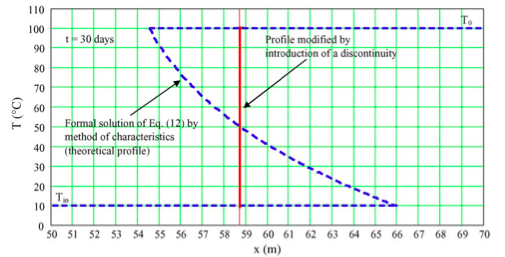
\includegraphics[width=4in]{np.png} 
   \caption{Non physical solution obtained in \cite{Waj05} from the method of characteristics}
   \label{fig:nonp}
\end{figure}

In this case The solution of equation (\ref{eq:cl3}) with initial data (\ref{eq:i}) see \cite{Waj05} is multivalued which mean that the solution is discontinuous. To obtain a physically acceptable solution, a discontinuity was inserted in the solution at position $z$ such that conservation of energy was satisfied see Figure \ref{fig:nonp}:

\begin{equation}\label{eq:cew}
t\frac{u_{w}}{\phi}\int_{u_{l}}^{u_{r}} U(u)F(u)\mathrm{d}u=z\int_{u_{l}}^{u_{r}} U(u)\mathrm{d}u
\end{equation}
setting $v_{TF}=\frac{z}{t}$ they obtained
\begin{equation}\label{eq:sw}
v_{TF} = \frac{u_{w}}{\phi}\left(   \frac{\int_{u_{l}}^{u_{r}} U(u)F(u)\mathrm{d}u   }{ \int_{u_{l}}^{u_{r}} U(u)\mathrm{d}u    }    \right) 
\end{equation}
\\
\begin{equation}\label{eq:u1}
U(u) =(1-\phi)\rho_{r}(u)(u)c_{r}(u) + \phi \rho_{w}(u)c_{w}(u).
\end{equation}
with $U(u)$ given in Figure \ref{fig:fu}. The thermal front velocity obtained by Stopa and Wajnarowski is the weighted average of the derivative of the flux function :

\begin{equation}\label{eq:G1}
G(u) = \frac{u_{w}}{\phi}\int_{0}^{u}F(x)\mathrm{d}x \implies  \frac{d G(u)}{d u}=\frac{u_{w}}{\phi}F(u)\nonumber
\end{equation}
So that (\ref{eq:sw}) ca be written as
\begin{equation}\label{eq:sw1}
v_{TF} = \left(   \frac{\int_{u_{l}}^{u_{r}} U(u)G^{\prime}(u)\mathrm{d}u   }{ \int_{u_{l}}^{u_{r}} U(u)\mathrm{d}u    }    \right) 
\end{equation}



\begin{figure}[H] %  figure placement: here, top, bottom, or page
   \centering
   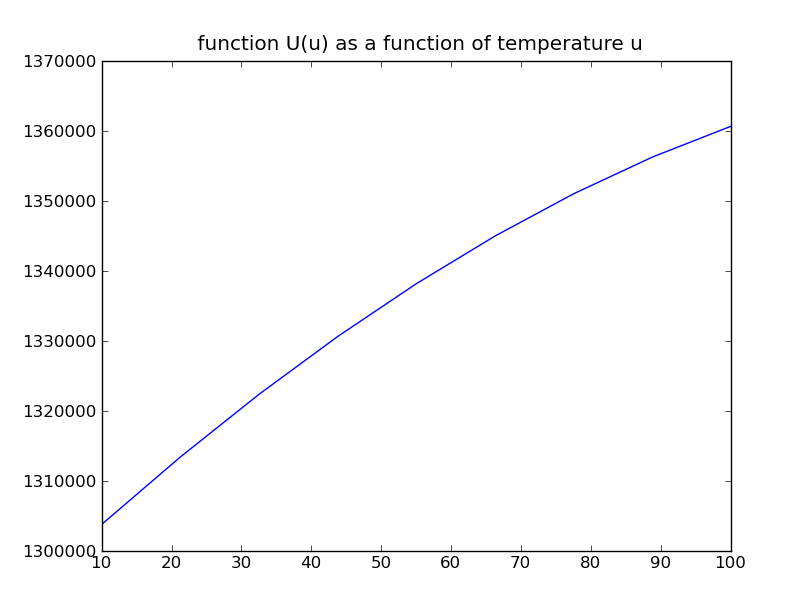
\includegraphics[width=4in]{fu.png} 
   \caption{Function $U$ given in \ref{eq:u1}}
   \label{fig:fu}
\end{figure}

%Equipped with results given in section 4.3 we are now ready to derive the thermal front velocity induced by injecting cold fluid into a hot geothermal reservoir. 

\subsection{Thermal front velocity predicted by the theory of conservation law}
Injecting colder water into a hot geothermal reservoir can be formulated as a Riemann problem : Find the unique weak solution $u$ of 
\begin{equation}\label{eq:rp}
\frac{\partial u}{\partial t} +\frac{ \partial G(u) }{\partial x}=0, \quad u(x,0)=g(x)
\end{equation}

\[ g(x) = \left\{ 
  \begin{array}{l l }
    u_{l} & \quad \text{if $x\leq 0$ }\\
    
    u_{r} & \quad \text{if $x\geq 0$ }.
  \end{array} \right.\]
satisfying the Rankine-Hugoniot shock condition and the Kruzkov entropy condition. The shock condition gives the speed $s$ of the discontinuity solution of (\ref{eq:rp}):

\begin{equation}\label{eq:rh}
s = \frac{G(u_{r})-G(u_{l})}{u_{r}-u_{l}}
\end{equation} 

The Kruzkov entropy condition:

\begin{equation}
\int_{0}^{T}\int_{-\infty}^{\infty}\left( \mid u-k \mid \varphi_{t}+q(u,k)\varphi_{x} \right) \mathrm{d}x \mathrm{d}t + \int \mid u(x,0)-k \mid \varphi(x,0) \mathrm{d}x  \geq 0 
\end{equation}
 is the extra condition satisfy by the unique solution of (\ref{eq:rp}) see \cite{Risebro07} for detail. $q(u,k)=sign(u,k)(G(u)-G(k))$, $k$ is a non negative constant and $\varphi$ is any non negative test function.\\
\\
From \cite{Risebro07}, the unique solution of (\ref{eq:rp}) satisfying the Rankine-Hugoniot condition and the Krizkov entropy condition is:


\begin{equation}
u(x,t) = \left\{
\begin{array}{rl}
u_{l} & \text{if } x \leq G^{\prime}_{\cup}(u_{l})t,\\
(G^{\prime}_{\cup})^{-1}(\frac{x}{t}) & \text{if }G^{\prime}_{\cup}(u_{l})t\leq x \leq G^{\prime}_{\cup}(u_{r})t\\
u_{r} & \text{if } x \geq G^{\prime}_{\cup}(u_{r})t
\end{array} \right.
\end{equation}
If $u_{l}<u_{r}$, and:
\begin{equation}
u(x,t) = \left\{
\begin{array}{rl}
u_{l} & \text{if } x \leq G^{\prime}_{\cap}(u_{l})t,\\
(G^{\prime}_{\cap})^{-1}(\frac{x}{t}) & \text{if }G^{\prime}_{\cap}(u_{l})t\leq x \leq G^{\prime}_{\cap}(u_{r})t\\
u_{r} & \text{if } x \geq G^{\prime}_{\cap}(u_{r})t
\end{array} \right.
\end{equation}
if $u_{l}>u_{r}$,
 where $G_{\cup},_\cap $ is the lower and the upper convex envelope of $G$ respectively.

%%%%%%%%%%%%%%%%%%%%%%%%%%%%%%%%%%%%%%%%%%%%%%%%%%%%%%%%%%%%%%%%%%%%%%%%%%%%%%%%%%%%%

%\subsection{Constant temperature rock and fluid properties}
%Assuming that the density and the heat capacity of rock and fluid are constant,  (\ref{eq:rp}) becomes
%
%\begin{equation}\label{eq:rpc}
% u_{t} +Fu_{x}=0, \quad u(x,0)=g(x)
%\end{equation}
%
%\[ g(x) = \left\{ 
%  \begin{array}{l l }
%    u_{l} & \quad \text{if $x\leq 0$ }\\
%    
%    u_{r} & \quad \text{if $x\geq 0$ }.
%  \end{array} \right.\]
%
%with 
%
%\begin{equation}\label{eq:Fc}
%F=\frac{   \phi \rho_{w} c_{w}     }{  (1-\phi)\rho_{r} c_{r} +  \phi \rho_{w}c_{w}     }
%\end{equation}
%
%We assume that the injected temperature $u_{l}$ is less then the reservoir temperature $u_{r}$. The unique solution $u$ is a shock moving at the speed $s$
%\[ u(x,t) = \left\{ 
%  \begin{array}{l l }
%    u_{l} & \quad \text{if $x\leq st$ }\\
%    
%    u_{r} & \quad \text{if $x\geq st$ }.
%  \end{array} \right.\]
%
%with $s$ given by the Rankine-Hugoniot shock condition 
%
%\begin{equation}
%\begin{aligned}
%s&=V_{w}\frac{G(u_{l})-G(u_{r})}{u_{l}-u_{r}}\\
%  &=\frac{Fu_{l}-Fu_{r}}{u_{l}-u_{r}}\\
%  &=F
%\end{aligned}
%\end{equation}
%
%Physically, a shock wave is a disturbance that induce abrupt change in the physical characteristic of the medium though which its propagates. When cold water is injected into the hot reservoir, at the interface between the cold water movement and the hot reservoir they is an abrupt change in temperature. This interface moves at the speed equal to $s$:
%\begin{equation}\label{eq:Fc}
%V_{TF}=s=V_{w}\frac{   \phi \rho_{w} c_{w}     }{  (1-\phi)\rho_{r} c_{r} +  \phi \rho_{w}c_{w}     }
%\end{equation}
%which is the cold front velocity.
%This result is the same as the one obtained by Bodvarsson \cite{Bod-R72} and Stoppa and Wajnarowski \cite{Waj05}, using the characteristics method. We should however note that the characteristics method fail to provide physically acceptable solution when the fluid and rock properties are temperature dependent \cite{Evan00}, \cite{Waj05}.
%
%%%%%%%%%%%%%%%%%%%%%%%%%%%%%%%%%%%%%%%%%%%%%%%%%%%%%%%%%%%%%%%%%%%%%%%%%%%%%%%%%%%
When fluid and rock properties depend continuously on temperature, The flux function $G$ is given by 
\begin{equation}
G(u) = V_{w}\int_{0}^{u} F(\theta)\mathrm{d}\theta\nonumber
\end{equation}

with 

\begin{equation}\label{eq:FF}
F(u)=\frac{  \phi \rho_{w}(u)\left(  \frac{\partial (c_{w}(u) u)  }{\partial u  }   \right)    }{  (1-\phi)\left( \frac{ \partial (\rho_{r}(u)  c_{r}(u) u) }{\partial u}\right) +  \phi \rho_{w}(u)\left(  \frac{\partial (c_{w}(u)u)  }{\partial u  } \right)     }
\end{equation}

\begin{figure}[H] %  figure placement: here, top, bottom, or page
   \centering
   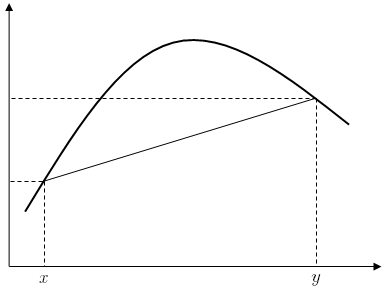
\includegraphics[width=2.7in]{G.png} 
      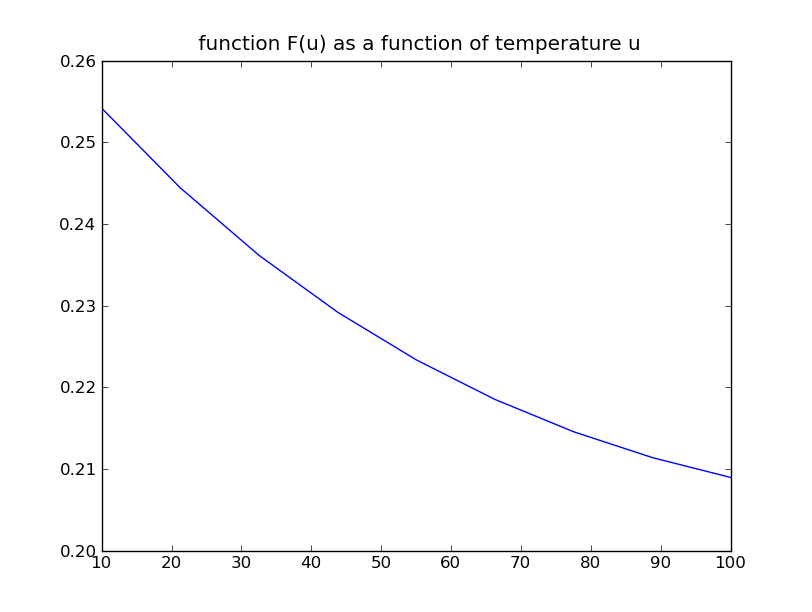
\includegraphics[width=2.7in]{F.png} 
   \caption{Function $F$ and $G$ with temperature $(x=u_{l}, y=u_{r})$}
   \label{fig:fg}
\end{figure}

From figure \ref{fig:fg} $F$ is monotonically decreasing on $[u_{l}=10,u_{r}=100]$, therefore the flux function $G$ is concave on that interval. The lower convex envelope $G_{\cup}$ of $G$  is the line passing through the points $(u_{l},G(u_{l}))$ and $(u_{r},G(u_{r}))$. In this case the unique solution of (\ref{eq:rp}) moving at the speed $s=V_{TF}$ is given by 

\[ u(x,t) = \left\{ 
  \begin{array}{l l }
    u_{l} & \quad \text{if $x\leq st$ }\\
    
    u_{r} & \quad \text{if $x\geq st$ }.
  \end{array} \right.\]
  
  \begin{figure}[htbp] %  figure placement: here, top, bottom, or page
     \centering
     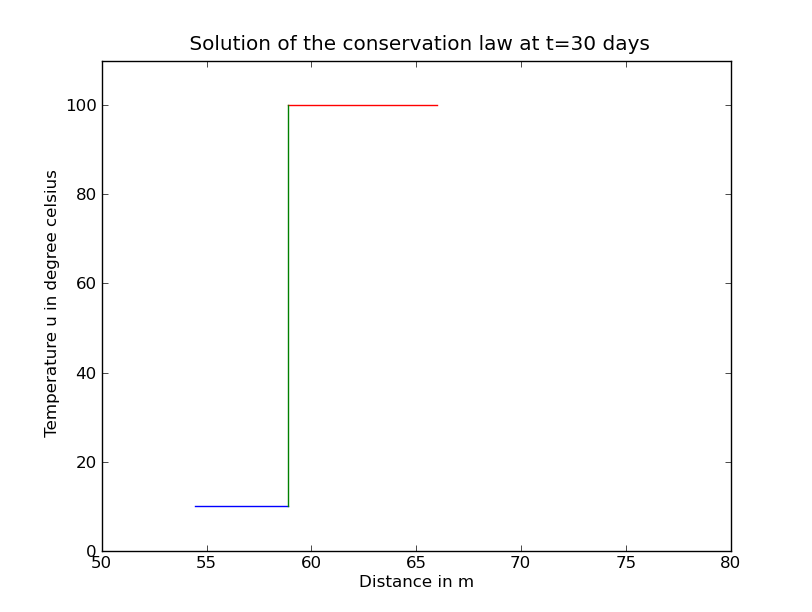
\includegraphics[width=4in]{u0.png} 
     \caption{Solution of \ref{eq:rp} at $t$ = 30 days}
     \label{fig:u0}
  \end{figure}
  with 
  $s=V_{TF}$ given by the Rankine-Hugoniot shock condition
  \begin{align}\label{eq:si}
s &=v_{TF} \nonumber \\
   &=\frac{  G(u_{l})-G(u_{r})   }{ u_{l}-u_{r} } \nonumber \\
  &=\frac{\frac{u_{w}}{\phi}}{(u_{r}-u_{l})}\left( \int_{0}^{u_{r}} F(u)\mathrm{d}u  - \int_{0}^{u_{l}} F(u)\mathrm{d}u \right)\nonumber \\
  &=\frac{\frac{u_{w}}{\phi}}{(u_{r}-u_{l})}\left( \int_{0}^{u_{l}} F(u)\mathrm{d}u +\int_{u_{l}}^{u_{r}} F(u)\mathrm{d}u   - \int_{0}^{u_{l}} F(u)\mathrm{d}u \right)\nonumber \\
  &=\frac{1}{(u_{r}-u_{l})}\left( \int_{u_{l}}^{u_{r}} \frac{u_{w}}{\phi}F(u)\mathrm{d}u   \right) 
\end{align}

\subsection{Numerical values and discussion}
In this section we compared numerically the values of the thermal front velocity from \cite{Waj05} and the theory of conservation laws. 
%Recall that the thermal front velocity $V_{TF}$ given in (\ref{eq:si}) differ from the one obtained in \cite{Waj05} in it expression. In the later, the method of characteristic was applied, resulting in a nonphysical solution. (see figure \ref{fig:np}). To obtain a physically acceptable solution, a discontinuity was inserted in the solution at position $z$ such that conservation of energy was satisfy:
%
%\begin{equation}\label{eq:cew}
%tv_{w}\int_{u_{l}}^{u_{r}} U(u)F(u)\mathrm{d}u=z\int_{u_{l}}^{u_{r}} U(u)\mathrm{d}u
%\end{equation}
%setting $v_{TF}=\frac{z}{t}$ they obtained
%\begin{equation}\label{eq:sw}
%v_{TF} = v_{w}\left(   \frac{\int_{u_{l}}^{u_{r}} U(u)F(u)\mathrm{d}u   }{ \int_{u_{l}}^{u_{r}} U(u)\mathrm{d}u    }    \right) 
%\end{equation}
%\\
%\begin{equation}\label{eq:u1}
%U(u) =(1-\phi)\rho_{r}(u)(u)c_{r}(u) + \phi \rho_{w}(u)c_{w}(u).
%\end{equation}
%with $U(u)$ given in Figure \ref{fig:fu}.
%
%\begin{figure}[H] %  figure placement: here, top, bottom, or page
%   \centering
%   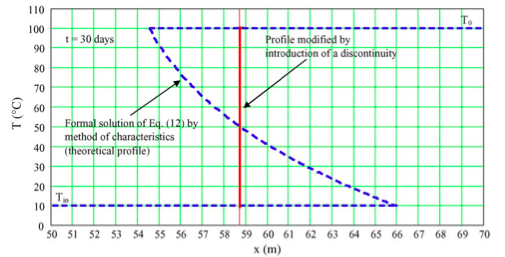
\includegraphics[width=4in]{np.png} 
%   \caption{Non physical solution obtained in \cite{Waj05} from the method of characteristics}
%   \label{fig:np}
%\end{figure}
%
%\begin{figure}[H] %  figure placement: here, top, bottom, or page
%   \centering
%   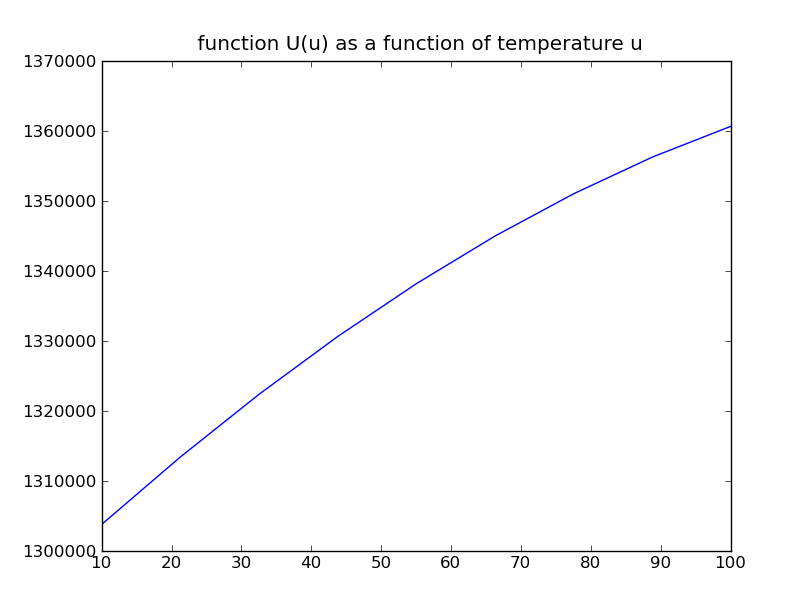
\includegraphics[width=4in]{fu.png} 
%   \caption{Function $U$ given in \ref{eq:u1}}
%   \label{fig:fu}
%\end{figure}


%%%%%%%%%%%%%%%%%%%%%%%%%%%%%%%%%%%%%%%%%%%%%%%%%%%%%%%%%%%%%%%%%%%%%%%%%%%%%%%%%%%
%\subsection{Numerical result}
%The trapezoidal rule from calculus state that the integral of a function $f$ on an interval $[a,b]$ can be approximated  by
%\\
%\begin{equation}\label{eq:trap}
%\int_{a}^{b}f(x) \mathrm{d}x \approx\frac{b-a}{2n}\left( f(a)+f(b)+\sum_{i=1}^{n-1}f(a+ih)\right)
%\end{equation}
%\\
%with absolute and asymptotic error (computable error) given respectively by
%
%\begin{equation}\label{eq:a}
%E_{n}^{a}=-\frac{h^{2}(b-a)}{12}(f^{\prime\prime}(c_{n}))
%\end{equation}
%and 
%
%\begin{equation}\label{eq:c}
%E_{n}^{c}=-\frac{h^{2}}{12}(f^{\prime}(b)-f^{\prime}(a))
%\end{equation}
%\\
%with some unknown $ c_{n} \in[a,b]$ and $ h = \frac{b-a}{n}$. Equation (\ref{eq:c}) is also called upper bound error and can also be written in terms of $n$ as 
%\\
%\begin{equation}\label{eq:cc}
%E_{n}^{c}=\frac{c}{n^{2}}
%\end{equation}
%with 
%
%\begin{equation}
%c=-\frac{(b-a)}{12}(f^{\prime}(b)-f^{\prime}(a)).\nonumber
%\end{equation}
%\\
%To evaluate the derivative of $f$ we use the finite difference approximation 
%\\
%\begin{equation}
%f^{\prime}(x)\approx \frac{f(x+h)-f(x-h)}{2h} \nonumber
%\end{equation}
%\\
%with approximation error given by
%\\
%\begin{equation}
%Err = \frac{1}{6}f^{\prime\prime\prime}h^{2}+O(h^{3}) = O(h^{2}).\nonumber
%\end{equation}
%
%
%
%
%
\begin{table}[H]
	\begin{center}
		\begin{tabular}{|l|c|c|c|r|}
		\hline
			$u_{l}$ & $u_{r}$ & [$V_{TF}$ from (\ref{eq:si}) ,$10^{-5}m/s$]& [$v_{TF}$ for (\ref{eq:sw}), $10^{-5}m/s$ ]&[$V_{TF}-v_{TF}$]  \\ \hline
			10 & 100 & $2.261$ & $2.257$  & $4*10^{-8}$   \\ 
			55 & 100 & $2.15$  & $2.15$       & $0.0  $    \\ 
			10 & 55 & $2.370$   & $2.369$    & $10^{-8}$  \\ 
			20 & 80 & $2.271$    & $2.269$  & $2*10^{-8} $ \\ 
			30 & 70 & $2.264$    & $2.263$    & $10^{-8} $ \\ 
			40 & 60 & $2.260$       &  $2.259$  & $10^{-8} $\\
			\hline
		\end{tabular}
		\caption{approximated values for evaluating (\ref{eq:si}) and (\ref{eq:sw})}
		\label{tab:ap}
	\end{center}
\end{table}
The thermal front velocity predicted by the theory of conservation laws is slimly higher than the one obtained by Stopa and Wajnaroski in \cite{Waj05}. A relative error of $10^{-3}$ is observed between the two results. 



%For symmetric and spherical flow problem, Bodvarsson presented a method to compute the radius of propagation of the thermal front velocity. Assume that a mass $M = Qt$ of fluid at time $t$ with temperature $u_{l}$ is injected at a flow rate $Q$ in a volume $V$ of reservoir rock with temperature $u_{r}$. If q is the magnitude of the mass flow vector of the fluid From \cite{Bod-R72}
%%we have the following relation
%\begin{equation}
%\frac{V}{Qt} = \frac{V_{TF}}{q} 
%\end{equation}
%
%For spherical symmetric flow the radius of propagation is 
%\begin{equation}
%r = \left(  \frac{3V_{TF}Qt}{4\pi q}         \right)^{\frac{1}{3}}
%\end{equation}
%and for cylindrical flow the radius of propagation is
%\begin{equation}
%r = \left(  \frac{V_{TF}Qt}{\pi q}         \right)^{\frac{1}{2}}
%\end{equation}
%
%\begin{figure}[htbp] %  figure placement: here, top, bottom, or page
%   \centering
%   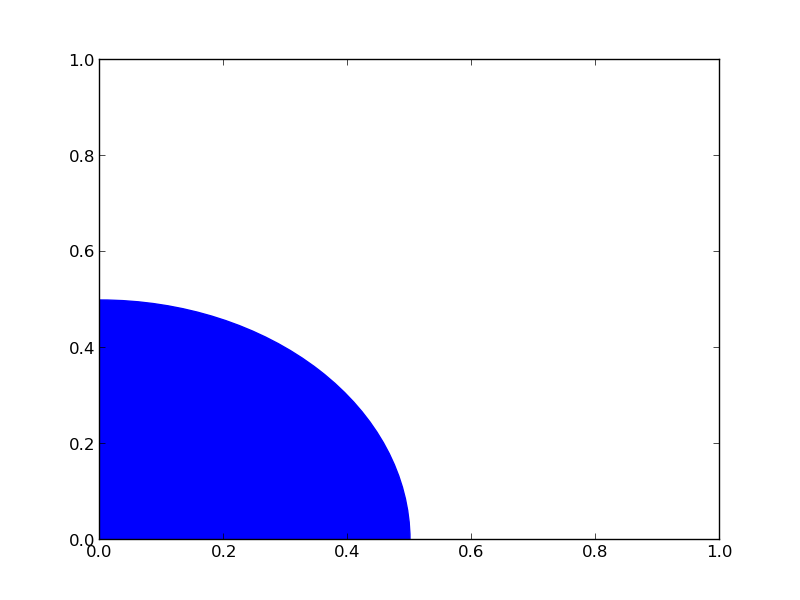
\includegraphics[width=2.5in]{waj.png}
%      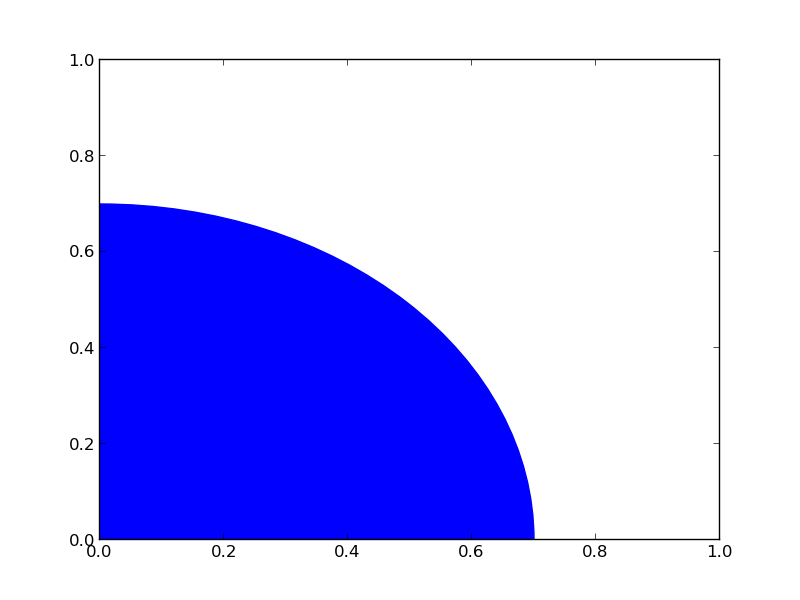
\includegraphics[width=2.5in]{cl.png} 
% 
%   \caption{Illustration of the radius of propagation for thermal front velocity from \ref{eq:sw} and \ref{eq:si}}
%   \label{fig:example}
%\end{figure}
%The radius of cold water propagation is therefore proportional to the thermal front velocity for spherical and cylindrical symmetric flow.
%
%\begin{table}[H]
%	\begin{center}
%		\begin{tabular}{|l|c|r|}
%		\hline
%			$n$ & Error for equation (\ref{eq:si}) & error for equation (\ref{eq:sw}) \\ \hline
%			10 & $5.6*10^{-5}$ & $174.6$ \\ 
%			40 & $4*10^{-6}$ & $10.9$ \\ 
%			70 & $10^{-6}$ & $3.5$ \\ 
%			107 & $0.0$ & $1.5$ \\ 
%			$10^{5}$ & $0.0$ & $1.2*10^{-5}$\\
%		\hline
%		\end{tabular}
%		\caption{Convergence test for the trapezoidal rule (\ref{eq:trap}) for equation (\ref{eq:si}) and (\ref{eq:sw})}
%		\label{tab:trapc}
%	\end{center}
%\end{table}
%
%
%Table \ref{tab:ap} shows that the values obtained by using either equation (\ref{eq:sw}) or (\ref{eq:si}) are equal within an error of $10^{-8}$. Table \ref{tab:trapc} indicates that the error in evaluating the integral in (\ref{eq:si}) converge to zero from $n=107$, while the error in evaluating the lower integral in equation (\ref{eq:si}) does not converge. To have convergence we are force to use a more accurate integration scheme such as Simpson (1/3) rule which is fourth order accurate. Using Simpson rule, the integral of a function $f$ is approximated by
%\\
%\begin{equation}\label{eq:sim}
%\int_{a}^{b}f(x) \mathrm{d}x \approx\frac{b-a}{3n}\left( f(a)+f(b)+4\sum_{i=1(odd)}^{n-1}f(a+ih)+ 2\sum_{i=2(even)}^{n-2}f(a+ih)\right)
%\end{equation}
%\\
%with computed or upper bound error given by
%\\
%\begin{equation}\label{eq:errs}
%E^{c}_{n} = -\frac{h^{4}}{180}(f^{\prime\prime\prime}(b)-f^{\prime\prime\prime}(a)).
%\end{equation}
%\\
%The third derivative of $f$ can be approximated by finite difference as 
%\\
%\begin{equation}
%f^{\prime}(x)\approx \frac{-\frac{1}{2} f(x-2h)+f(x-h)-f(x+h)+\frac{1}{2}f(x+2h)}{h^{3}} \nonumber
%\end{equation}
%\\
%
%\begin{table}[H]
%	\begin{center}
%		\begin{tabular}{|l|c|r|}
%		\hline
%			$n$ & Error for equation (\ref{eq:si}) & error for equation (\ref{eq:sw}) \\ \hline
%			10 & $5.6*10^{-5}$ & $72975$ \\ 
%			50 & $4*10^{-6}$ & $116.76$ \\ 
%			176 & $0.0$ & $0.76$ \\ 
%			6000 & $0.0$ & $10^{-6}$ \\ 
%			$6181$ & $0.0$ & $0.0$\\
%		\hline
%		\end{tabular}
%		\caption{Convergence test for Simpson (1/3) rule (\ref{eq:sim}) for equation (\ref{eq:si}) and (\ref{eq:sw})}
%		\label{tab:sim}
%	\end{center}
%\end{table}
%
%
%\begin{table}[H]
%	\begin{center}
%		\begin{tabular}{|l|c|c|c|r|}
%		\hline
%			a & b & [$V_{TF}$ from (\ref{eq:si}) ,$10^{-5}m/s$]& [$v_{TF}$ for (\ref{eq:sw}), $10^{-5}m/s$ ]&[$V_{TF}-v_{TF}$]  \\ \hline
%			10 & 100 & $2.261$ & $2.257$  & $4*10^{-8}$   \\ 
%			55 & 100 & $2.15$  & $2.15$       & $0.0  $    \\ 
%			10 & 55 & $2.370$   & $2.369$    & $10^{-8}$  \\ 
%			20 & 80 & $2.271$    & $2.269$  & $2*10^{-8} $ \\ 
%			30 & 70 & $2.264$    & $2.263$    & $10^{-8} $ \\ 
%			40 & 60 & $2.260$       &  $2.260$  & $0.0 $\\
%			\hline
%		\end{tabular}
%		\caption{approximated values for evaluating (\ref{eq:si}) and (\ref{eq:sw}) using (\ref{eq:sim})}
%		\label{tab:aps}
%	\end{center}
%\end{table}
%
%\begin{table}[H]
%	\begin{center}
%		\begin{tabular}{|lc|c|c|r|}
%		\hline
%			n& $E_{1}$ ($10^{-6}$) &$E_{2}$&$E_{3}$ &convergence rate  \\ \hline
%			4 & $351$& $663.35$ & $469.2$   & $(E_{1})$: $[1.99,2.01,1.98]$   \\ 
%			5& $225$ & $425.5$  & $300.31$  & $(E_{2})$: $[2.00,1.99,2.02]   $    \\ 
%			6 & $156$ & $294.8$   & $208.5$   & $(E_{3})$: $[1.99,2.00,1.99] $  \\ 
%			7 & $115$ & $216$    & $153.2$  & \\
%			
%			\hline
%		\end{tabular}
%		\caption{Convergence rate for the error in the trapezoidal rule}
%		\label{tab:apr}
%	\end{center}
%\end{table}
%
%
%In Table \ref{tab:apr} $E_{1}$ represent the upper bound error in evaluating \ref{eq:si}, $E_{2}$ represent the upper bound error in evaluating the upper integral of \ref{eq:sw} and $E_{3}$ the upper bound error in evaluating the lower integral. The rate of convergence is bout 2, which is the same as the error for the trapezoidal rule. This shows that the numerical results obtained using the trapezoidal rule are accurate.\\ 
%Table \ref{tab:aps} shows the result obtained using Simpson $(1/3)$ rule. This result is similar to the one obtained in table \ref{tab:ap} except in the last entry of the tables. The largest difference between the result obtained from \cite{Waj05} and the theory of conservation laws is an order of $10^{-8}$. 

%\section{discussion}
%For temperature dependent fluid and rock properties, the mass and energy equation for fluid flow in porous medium can be reduced to a conservation laws when heat conduction is neglected. In this case, injecting colder water into a hot geothermal reservoir can be solve as a Riemann problem  for the conservation laws. The thermal front velocity coincide with the velocity of the discontinuity solution satisfying the Kruzkov entropy solution \cite{Risebro07}. Our result was compared with the result obtained in \cite{Waj05}. in the later, starting with a nonphysical solution, a discontinuity was inserted into the solution such that the new physical acceptable solution satisfies the conservation of energy entropy condition.                  
%A numerical simulation showed that the error in evaluating the thermal front velocity from our result goes rapidly to zero compared with the error in evaluating the thermal front velocity obtained in \cite{Waj05}.

%Thermal front or cold injected front is the interface between the cold injected fluid and the hot reservoir. At this interface, temperature changes very rapidly between injected fluid temperature and reservoir temperature. To capture this mathematically, a jump discontinuity is inserted at this interface. As cold water flows through the reservoir, the jump discontinuity position moves as well. Its position at any time gives the position of the cold moving front. \\
%Our computed thermal front velocity agrees with the one obtained in \cite{Bod-R72} for temperature independent rock and fluid properties event though different method were used. For temperature dependent fluid and rock properties, Our result and the one in \cite{Waj05} were numerically closed. However our method is based on a well established theory of hyperbolic conservation laws described in \cite{Risebro07}. The Riemann problem upon which we derived the thermal front velocity is well posed \cite{Risebro07}.\\ 
%A numerical solution of the conservation laws using a stabilised numerical scheme for conservation laws, could be used to simulate cold front propagation to further this work.
%This work could also be extended to the case where hot water is injected to a colder reservoir.  


